\chapter{Konzept}
Die Algorithmen und Prozesse einer Filialplanung spiegeln sehr gut einen allgemeinen Anwendungsfall moderner GIS. 
Neben einer einfachen Hintergrundkarte sind die Mitarbeiter auf Zeichenwerkzeuge, Geo-Daten-Anzeige, thematische Karten und Kennzahlen Berechnungen angewiesen, um akkurate und fundierte Prognosen und Planungen treffen zu können.
Viele theoretische Konzepte und Prozesse passieren hierbei im Hintergrund und sind nicht direkt ersichtlich.
In den folgenden Kapiteln werden die wichtigsten Beschrieben mit dem Fokus auf den Algorithmus der hinter dem Gravitations-Model von Huff steht.
\section{Algorithmen und Prozesse}
Um eine realistische Abbildung der Welt auf eine Karte zu bringen benötigt es eine Umrechnung eines Ovales, quasi der Erdkugel, auf eine Rechteck, im Fall eines Web-Gis des Bildschirms. 
\subsection{Gravitations-Modelle}
Das \textit{Huff-Modell} (engl. Huff Gravitation Model) ist ein mathematisches Modell zur Abgrenzung und Segmentierung von Marktgebieten \cite{Roy2004}.
Das Modell bestimmt die Wahrscheinlichkeit, mit der Kunden einen Standort (Filiale, Einkaufszentrum) in Abhängigkeit von Distanz und Attraktivität aufsuchen. 
Die Formel wird im allgemeinen wie folgt dargestellt:

\begin{figure}
	\centering
	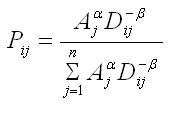
\includegraphics[]{resources/images/huff_model}
	\label{img:huff_formula}
\end{figure}

Die Wahrscheinlichkeiten werden nun auf der Karte als Punkte dargestellt, die rund um den Standort platziert werden. 
Die Punkte der selben Wahrscheinlichkeiten werden zu Isowahrscheinlichkeitslinien verbunden. 
So entstehen zu jedem Standort verschiedene Gravitationsebenen, die farblich gekennzeichnet werden. 
Die Beeinflussung der verschiedenen Gravitationsebenen führt zu mehreren Farbverläufen, die ein komplexes Bild der Standort Landschaft bilden.
In seiner einfachsten Form berücksichtigt das Modell nur die Distanz und eine simple Kennzahl der Attraktivität (zum Beispiel in Form eines Rankings) für die Wahrscheinlichkeitsberechnung. 
Hierzu wird zunächst ein maximaler Einflussbereich der Filialstandorte definiert. 
Dieser Bereich stellt die Grundlage der Berechnungen dar und muss deswegen bekannt und mit berechenbaren Kennzahlen gefüllt sein.
Zur Bestimmung des Bereiches können einfache geografische Abstände oder Gebiete benutzt werden, wie zum Beispiel eine Berechnung auf Grundlage Berlins als Einflussbereichs.
Vor Allem aber kommen zeitliche oder örtliche Parameter zum Einsatz.
So macht es aus wirtschaftlicher Sicht viel mehr Sinn das Gebiet anhand von Fahrzeitzonen zu berechnen.
So würde ein potenzieller Kunde aus Brandenburg wahrscheinlich auch in einer Filiale in Berlin einkaufen gehen, wenn diese attraktiver, örtlich näher oder besser zu erreichen ist.
Berechnet wird also ein Einzugsbereich, um die Filiale herum.
Ob dies nun eine maximale Fahrtzeit von 30 Minuten ist oder eher eine maximale Distanz von 30 Kilometern, ist auf die einzelne Filiale oder den gewählten Standard der Berechnung zurückzuführen.

Um die Huff-Formel korrekt kalibrieren zu können, genauer gesagt die Parameter alpha und beta empirisch bestimmen zu können, müssen folgende Schritte befolgt werden:

\begin{itemize}
	\item Abgrenzung des Erhebungsgebiets
	\item Unterteilung des Erhebungsgebiets in Untergebiete
	\item Zentroiden der Gebiete festlegen
	\item Alle konkurrierende Einrichtungen identifizieren und Koordinaten erfassen
	\item Entfernungen zwischen den Zentroiden aller Gebiete und aller Einrichtungen berechnen
	\item Spezifizieren aller Eigenschaften zur Kundenbeeinflussung
	\item Wirtschaftliche, soziale und demografische Daten für Gebiete angeben
	\item Studie durchführen für die Frequenz in welcher Kunden Einrichtungen besuchen
\end{itemize}

Einwohner pro Gebiet berechnen = Größe mal Faktor 0,006

Kaufkraft der gebiete = Einwohner mal durchschnittliche Kaufkraft Berlin (21,687€) Quelle https://de.statista.com/statistik/daten/studie/168591/umfrage/kaufkraft-nach-bundeslaendern/

Ausgaben für Lebensmittel = Einwohner mal durchschnittliche Ausgaben für Lebensmittel (356 € Quelle https://www.destatis.de/DE/Themen/Gesellschaft-Umwelt/Einkommen-Konsum-Lebensbedingungen/Konsumausgaben-Lebenshaltungskosten/Tabellen/privater-konsum-d-lwr.html;jsessionid=848A137E8A70CBDB1F7FD40382B122EE.internet8721)


Weiterführend muss bestimmt werden wie und ob sich das Potenzial über den Verlauf der Distanz des Einzugsbereiches verändert.
Bleibt das Potenzial konstant, würde dies bedeuten die Kunden in den äußeren Bereichen des Gebiets kommen mit der gleichen Wahrscheinlichkeit in die Filiale wie die Kunden in den unmittelbar angrenzenden Bereichen.
Aber gegenteilig wäre ein linear abnehmendes Potenzial wahrscheinlich ebenso nicht vollständig realitätsgetreu, da Kunden ab einer Distanz, die zu groß für den Fuß-Weg wäre, eher das Auto oder den öffentlichen Nahverkehr wählen und dann eventuell direkt zu einer attraktiveren Filiale weiter weg fahren würden. 
Daher kann als grundlegende Distanzfunktion quasi eine beliebig komplizierte Formel gewählt werden.
Aus Gründen der Vereinfachung und Demonstration wird für den Prototyp eine einfache linear abnehmende Distanzfunktion gewählt.

Nachdem nun zunächst die Potenzialberechnung für eine einzelne Filiale anhand der beschriebenen Parameter und Funktionen erfolgen konnte gilt es nun das Potenzial in einem bestehendem Filialnetz zu berechnen.
Als Ergebnis wird hierbei eine Wahrscheinlichkeitsberechnung für sämtliche Filialen des Netzes erwartet, sodass jedem Feld des summierten Gesamt-Einzugsgebietes einen Wahrscheinlichkeitswert zugeordnet werden kann, der beeinflusst von sämtlichen anderen Filialen des Netzes, für jede Filiale des Netzes unterschiedlich sein kann und dementsprechend eingefärbt werden kann.
Das Endergebnis zeigt somit die beschriebene farbliche Gravitationskarte.

Für die komplexere Berechnung mit mehr Faktoren wird das MCI-Modell von Nakanishi und Cooper verwendet, welches die Weiterentwicklung der einfachen Huff-Modells darstellt \cite{mciModell}.

Das \textit{MCI-Modell} ...
\section{Architektur}
